\documentclass[border=10pt]{standalone}
\usepackage{tikz}
\usepackage{amsmath}
\usetikzlibrary{positioning, arrows.meta, fit, backgrounds, shapes.geometric, calc}

% Architecture of the visual model at deployment (inference) time.
% Training-only components (loss terms) are described in the Training chapter
% and are therefore not shown here. Symbols follow the Methodology chapter.

\begin{document}
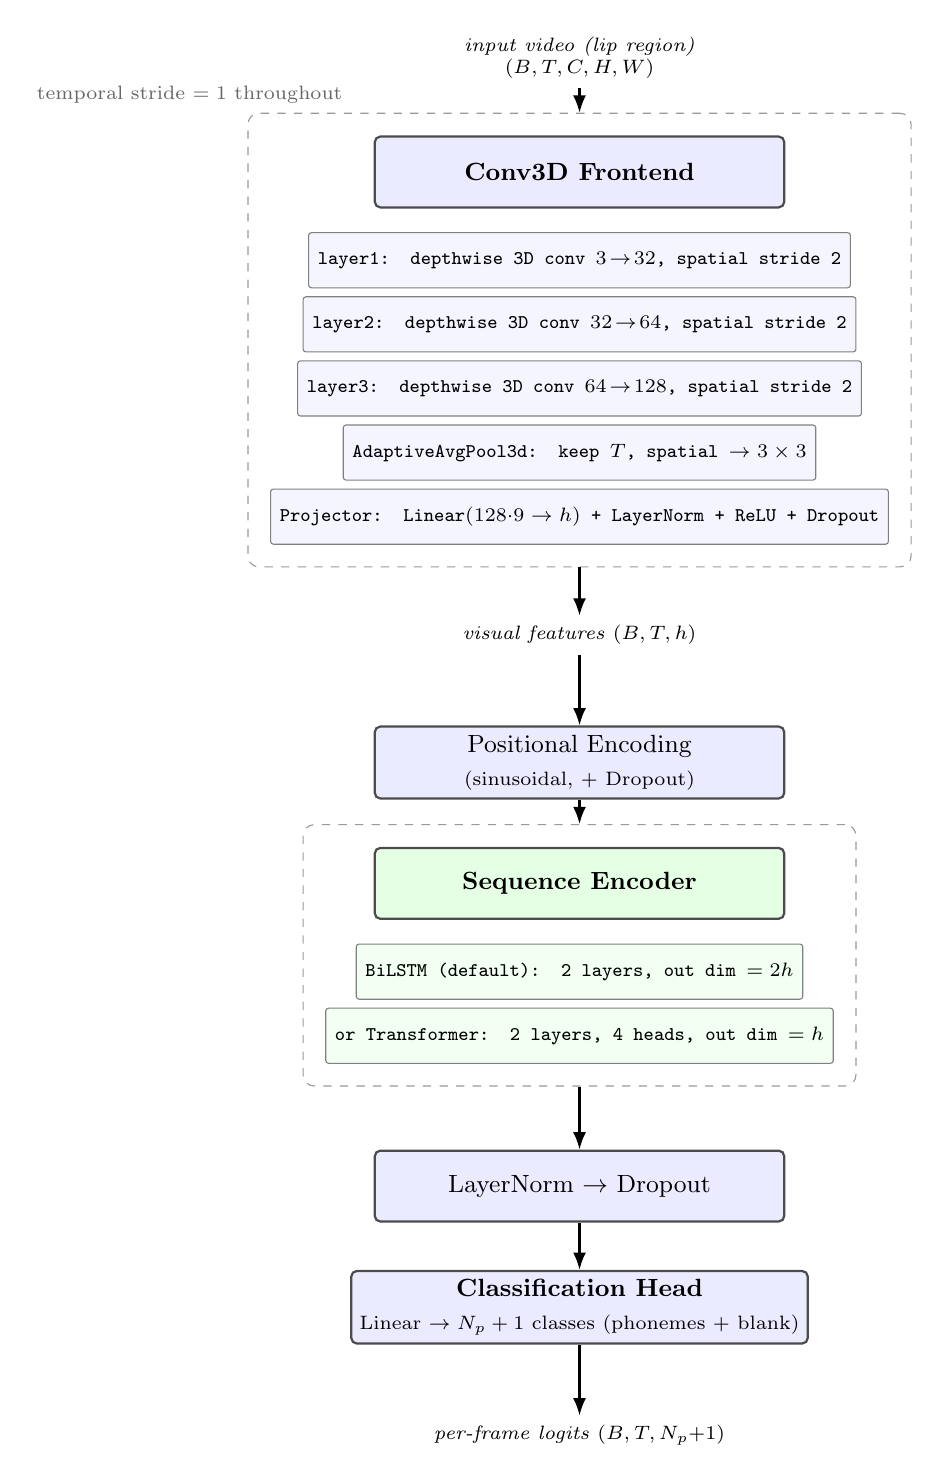
\begin{tikzpicture}[
    font=\small,
    node distance=6mm and 14mm,
    block/.style={
        rectangle, draw=black!70, thick, rounded corners=2pt,
        fill=blue!8, minimum width=52mm, minimum height=9mm,
        align=center, inner sep=3pt
    },
    subblock/.style={
        rectangle, draw=black!50, rounded corners=1pt,
        fill=blue!4, minimum width=46mm, minimum height=7mm,
        align=center, font=\scriptsize\ttfamily
    },
    iolabel/.style={
        rectangle, draw=none, fill=none, align=center, font=\scriptsize\itshape
    },
    groupbox/.style={
        rectangle, draw=black!40, dashed, rounded corners=4pt, inner sep=8pt
    },
    arr/.style={-{Latex[length=2.2mm]}, thick},
    every label/.style={font=\scriptsize}
]

% ---------------- Input ----------------
\node[iolabel] (input_lbl) {input video (lip region)\\ $(B, T, C, H, W)$};

% ---------------- Conv3D Frontend ----------------
\node[block, below=of input_lbl] (frontend_title) {\textbf{Conv3D Frontend}};
\node[subblock, below=3mm of frontend_title] (l1) {layer1: depthwise 3D conv $3\!\to\!32$, spatial stride 2};
\node[subblock, below=1mm of l1] (l2) {layer2: depthwise 3D conv $32\!\to\!64$, spatial stride 2};
\node[subblock, below=1mm of l2] (l3) {layer3: depthwise 3D conv $64\!\to\!128$, spatial stride 2};
\node[subblock, below=1mm of l3] (pool) {AdaptiveAvgPool3d: keep $T$, spatial $\to 3\times3$};
\node[subblock, below=1mm of pool] (proj) {Projector: Linear$(128{\cdot}9\to h)$ + LayerNorm + ReLU + Dropout};

\node[groupbox, fit=(frontend_title)(l1)(l2)(l3)(pool)(proj), label={[font=\scriptsize,text=black!60]above left:temporal stride $=1$ throughout}] (frontendbox) {};

\node[iolabel, below=9mm of proj] (feat_lbl) {visual features $(B, T, h)$};

% ---------------- Positional Encoding ----------------
\node[block, below=9mm of feat_lbl] (posenc) {Positional Encoding\\[1pt] \scriptsize (sinusoidal, + Dropout)};

% ---------------- Sequence Encoder (two variants) ----------------
\node[block, below=of posenc, fill=green!10] (enc_title) {\textbf{Sequence Encoder}};
\node[subblock, below=3mm of enc_title, fill=green!5] (bilstm) {BiLSTM (default): 2 layers, out dim $=2h$};
\node[subblock, below=1mm of bilstm, fill=green!5] (transformer) {or Transformer: 2 layers, 4 heads, out dim $=h$};
\node[groupbox, fit=(enc_title)(bilstm)(transformer)] (encbox) {};

\node[block, below=8mm of encbox] (norm) {LayerNorm $\to$ Dropout};

\node[block, below=of norm] (classifier) {\textbf{Classification Head}\\[1pt] \scriptsize Linear $\to N_p+1$ classes (phonemes + blank)};

\node[iolabel, below=9mm of classifier] (logits_lbl) {per-frame logits $(B, T, N_p{+}1)$};

% ---------------- Arrows ----------------
\draw[arr] (input_lbl) -- (frontendbox);
\draw[arr] (frontendbox.south) -- (feat_lbl.north);
\draw[arr] (feat_lbl.south) -- (posenc.north);
\draw[arr] (posenc) -- (encbox);
\draw[arr] (encbox) -- (norm);
\draw[arr] (norm) -- (classifier);
\draw[arr] (classifier.south) -- (logits_lbl.north);

\end{tikzpicture}
\end{document}
